\documentclass[a5paper,10pt]{article}
\usepackage[left=1cm,right=1cm,top=1.5cm,bottom=1cm]{geometry}

\usepackage{amsmath, amssymb}
\usepackage{mathtools}
\usepackage{titling}
\usepackage{fancyhdr}
\usepackage[inline]{enumitem}
\usepackage{changepage}
\usepackage{cancel,nicefrac}
\usepackage{dirtytalk}
\usepackage[svgnames]{xcolor}
\usepackage{graphicx,wrapfig}
\usepackage{tikz}
\usetikzlibrary{calc,patterns,arrows.meta}
\usetikzlibrary{decorations.markings,plotmarks}
\usepackage{tkz-euclide}
\usepackage[small]{titlesec}% Change sections font size
\usepackage[version=4,textfontname=sffamily]{mhchem}
\usepackage{chemfig}

\usepackage[T1]{fontenc}
\usepackage{libertine}

% Document setup
\newcommand{\assignmentauthor}{github/3fxcf9}
\newcommand{\assignmentdate}{Baccalaureat 2024}
\newcommand{\assignmenttitle}{Chimie}

% Header and Footer setup
\pagestyle{fancy}
\fancyhf{}
\fancyhf[lh]{\assignmentauthor}
\fancyhf[ch]{\itshape\assignmenttitle}
\fancyhf[rh]{\assignmentdate}
\fancyhf[rf]{\thepage}

% Line spacing
\titlespacing*{\section}{0pt}{0.1\baselineskip}{0.2\baselineskip}
\titlespacing*{\subsection}{0pt}{0.1\baselineskip}{0.2\baselineskip}

% Usefull commands
\newcommand{\N}{\mathbb{N}}
\newcommand{\Z}{\mathbb{Z}}
\newcommand{\R}{\mathbb{R}}
\renewcommand{\P}{\mathbb{P}}
\renewcommand*{\vec}{\overrightarrow}

\begin{document}
\renewcommand{\headsep}{10pt}
\thispagestyle{empty}
\vspace*{-1cm}
\noindent\assignmentauthor \hfill \assignmentdate
\vspace{-6pt}
\begin{center}
    \rule[2ex]{\textwidth}{1pt}\\
    \vspace{-4pt}
    {\Large{\assignmenttitle}}
    \vspace{-4pt}
\end{center}
\rule[2ex]{\textwidth}{1pt}\\
\title{}
\author{}
\date{}
\vspace{-0.5cm}

\section{Réactions d'oxydoréduction}
\subsection{Définitions}
\textbf{Oxydant}: Espèce chimique capable de capter au moins un electron (\textbf{réducteur} = céder).\\
\textbf{Demi-équation redox}: \ce{Ox + ne- <=> Red}\\
\textbf{Réaction redox}: Trans. d'electron(s) entre le red. d'un couple et l'ox. d'un autre.

\subsection{Ajustement d'une demi-équation d'oxydoréduction}
\begin{adjustwidth}{10pt}{0pt}
    \begin{enumerate*}[noitemsep, label=\textbf{\arabic*}.]
        \item Conservation des atomes autres que \ce{H} et \ce{O}.\phantom{text}
        \item Conservation de l'oxygène (\ce{H2O}).\\
        \item Conservation de l'hydrogène (\ce{H+}).\phantom{textnrsuietrn}
        \item Conservation des charges.
    \end{enumerate*}\\
\end{adjustwidth}

\section{Transformations acide-base}
\subsection{Définitions}
\textbf{Acide}: Espèce chimique capable de céder au moins un ion \ce{H+} (noté \textbf{\ce{AH}}).\\
\textbf{Base}: Espèce chimique capable de capter au moins un ion \ce{H+} (noté \textbf{\ce{A-}}).\\
\textbf{Couple acide/base}: Un acide et une base capables de s'échanger au moins un ion \ce{H+}.\\
\textbf{Demi-équation acido-basique}: Lie un acide à sa base conjuguée. (\textbf{\ce{AH <=> A- + H+}}).\\
\textbf{Réaction acido-basique}: Met et jeu deux couples A/B échangeant au moins un ion \ce{H+}.

\subsection{Exemples à retenir}
\textbf{\ce{HCl}} (Chlorure d'hydrogène) | \textbf{\ce{CH3-COOH}} (Acide éthanoïque\footnote{Aussi appelé \textit{acide acétique}}) | \textbf{\ce{NH4+}} (Ion ammonium).\\
\textbf{\ce{CH3-COO-}} (Ion éthanoate/acétate) | \textbf{\ce{NH3}} (Ammoniac)\\
\textbf{\ce{H3O+/H2O}} (Couple ion oxonium/eau) | \textbf{\ce{H2O/HO-}} (Couple eau/ion hydroxyde)\footnote{L'eau est une espèce \textit{amphotère} (ou un \textit{ampholyte}), à la fois l'acide d'un couple et la base d'un autre.}.

\subsection{pH d'une solution aqueuse}
Il est lié à la présence d'ions oxonium (\ce{H3O+}) dans la solution:
$$pH=-log\left(\frac{[\text{\ce{H3O+}}]}{C_0}\right) \iff [\text{\ce{H3O+}}]=C_0\times 10^{-pH}$$
Où $C_0=1\text{mol}\cdot \text{L}^{-1}$.

\subsection{Quotient de réaction et constante d'équilibre}
Le \textit{quotient de réaction} à un instant donné de la réaction \ce{aA + bB <=> cC + dD} vaut:
$$Qr=\frac{\left(\frac{[\text{\ce{C}}]}{C_0}\right)^c \times \left(\frac{[\text{\ce{D}}]}{C_0}\right)^d}{\left(\frac{[\text{\ce{A}}]}{C_0}\right)^a \times \left(\frac{[\text{\ce{B}}]}{C_0}\right)^b}$$
Les solides et les solvants interviennent par le chiffre 1. À l'équilibre, le quotient de réaction d'une réaction dépend uniquement de la température. On l'appelle $K$:
$$K=Qr_{\text{éq}}$$

\subsection{Produit ionique de l'eau}
L'eau est un ampholyte, toute solution aqueuse contient donc des ions \ce{H3O+} et \ce{HO-}.\\
La constante d'équilible $K_e$ de cette réaction d'\textit{autoprotolyse} vaut:
$$K_e=\frac{[\text{\ce{H3O+}}]}{C_0}\times \frac{[\text{\ce{HO-}}]}{C_0}$$
En particulier, pour toute solution aqueuse à 25\textcelsius, $K_e=10^{-14}$ et $pK_e=-log(K_e)=14$.\\
Dans l'eau pure et dans toute solution neutre, $[\text{\ce{H3O+}}]=[\text{\ce{HO-}}]$, on a donc:
$$pK_e=-log([\text{\ce{H3O+}}]^2)=-2\cdot log([\text{\ce{H3O+}}])=2\cdot pH \iff pH=\frac{1}{2}pK_e=7$$

\subsection{Force des acides et des bases}
On classe les acides et les bases dans deux familles: les acides/bases forts et les acides/bases faibles.
Un acide/base fort réagit completement avec l'eau ($\tau\approx 1$) ce qui n'est pas le cas des acides/bases faibles ($\tau < 1$).
Pour les classer, on peut comparer la concentration $C$ en acide/base apportée à la concentration en ions oxonium/hydroxyde à l'équilibre.\\
Pour un acide fort, on a $pH=-log(C)$ et pour une base forte:
$$pH=-log([\text{\ce{H3O+}}])=-log\left(\frac{K_e}{[\text{\ce{HO-}}]}\right)=-log\left(\frac{K_e}{C}\right)=log(C)-log(Ke)$$

\subsection{Constante d'acidité d'un couple acido-basique}
La constante d'acidité $K_A$ d'un couple acide/base faible est la constante d'équilibre de la réaction \ce{AH + H2O <=> A- + H3O+}:
$$K_A=\frac{\frac{[\text{\ce{A-}}]_{\text{eq}}}{C_0} \times \frac{[\text{\ce{H3O+}}]_{\text{eq}}}{C_0}}{\frac{[\text{\ce{AH}}]_{\text{eq}}}{C_0}};\quad pK_A=-log(K_A)$$
Plus la valeur de $K_A$ est grande (plus celle $pK_A$ est petite), plus l'avancement de la réaction est grand et donc plus l'acide est fort.
L'acide le plus fort en s° aq. est \ce{H3O+} ($pK_A=0$).

\subsection{Domaines de prédominances}
Pour tout couple acide/base:
$$pH=-log\left([\text{\ce{H3O+}}]\right)=-log\left(\frac{Ka\times [\text{\ce{AH}}]}{[\text{\ce{A-}}]}\right)=pK_A+log\left(\frac{[\text{\ce{A-}}]_{\text{eq}}}{[\text{\ce{AH}}]_{\text{eq}}}\right)$$
D'après cette relation, on peut envisager les trois situations suivantes:
\begin{itemize}[noitemsep]
  \item L'\hspace*{1pt}acide du couple prédomine: $\frac{[\ce{A-}]}{[\ce{AH}]}<1 \iff log\left(\frac{[\text{\ce{A-}}]_{\text{eq}}}{[\text{\ce{AH}}]_{\text{eq}}}\right)<0 \iff pH<pK_A$
  \item La base du couple prédomine: $\frac{[\text{\ce{A-}}]}{[\text{\ce{AH}}]}>1 \iff log\left(\frac{[\text{\ce{A-}}]_{\text{eq}}}{[\text{\ce{AH}}]_{\text{eq}}}\right)>0 \iff pH>pK_A$
  \item A/B en concentrations égales: $\frac{[\text{\ce{A-}}]}{[\text{\ce{AH}}]}=1 \iff log\left(\frac{[\text{\ce{A-}}]_{\text{eq}}}{[\text{\ce{AH}}]_{\text{eq}}}\right)=0 \iff pH=pK_A$
\end{itemize}

\subsection{Indicateurs colorés}
\textit{Un indicateur coloré (IC) acido-basique est un couple Acide/Base noté IndH/Ind- dont les especes conjuguées n'ont pas la même couleur}
(repérer équivalence, dosage colorimétrique).

\subsection{Solution tampon}
\textit{Une solution tampon est une solution dont le pH varie peu par dilution ou ajout de petites quantités de solutions acides ou basiques.}

\subsection{Acides $\alpha$-aminés}
\textit{Un acide $\alpha$-aminé contient un groupe carboxyle \ce{-COOH} et un groupe amine \ce{-NH3}. En solution aqueuse, il se forme un amphion, espèce aphotère.}\\[4pt]
Dans l'exemple ci-dessous, on remarque le caractère \textit{amphotère} de l'amphion: il fait partie de deux couples un avec le cation, l'autre avec l'anion.\\
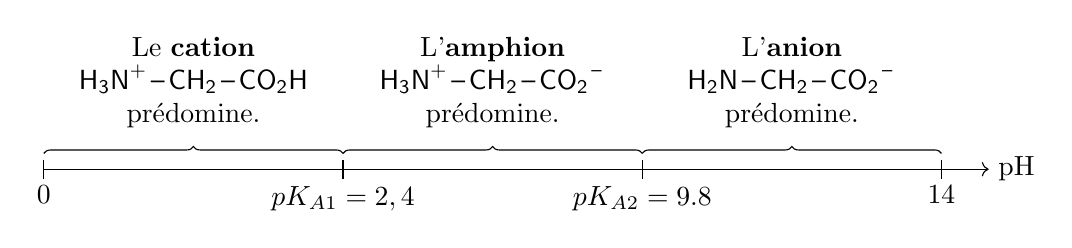
\begin{tikzpicture}
    \draw[->] (0,0) -- ++(12,0) node[right] {pH};

    \draw (0,-0.12) -- ++(0,0.24) node[below=6pt] {0};
    \draw (3.8,-0.12) -- ++(0,0.24) node[below=6pt] {$pK_{A1}=2,4$};
    \draw (7.6,-0.12) -- ++(0,0.24) node[below=6pt] {$pK_{A2}=9.8$};
    \draw (11.4,-0.12) -- ++(0,0.24) node[below=6pt] {14};

    \draw [
        decoration={
                brace,
                raise=0.2cm
            },
        decorate
    ] (0,0) -- (3.8,0) node[above=0.4cm, midway, align=center] {Le \textbf{cation}\\\ce{H3N+-CH2-CO2H}\\prédomine.};
    \draw [
        decoration={
                brace,
                raise=0.2cm
            },
        decorate
    ] (3.8,0) -- (7.6,0) node[above=0.4cm, midway, align=center] {L'\textbf{amphion}\\\ce{H3N+-CH2-CO2-}\\prédomine.};
    \draw [
        decoration={
                brace,
                raise=0.2cm
            },
        decorate
    ] (7.6,0) -- (11.4,0) node[above=0.4cm, midway, align=center] {L'\textbf{anion}\\\ce{H2N-CH2-CO2-}\\prédomine.};
\end{tikzpicture}

\section{Méthodes chimiques d'analyse}
\subsection{Titre massique}
La concentration $C$ d'une solution peut être déterminée à l'aide de son pourcentage massique $P_E$ et de sa densité $d$:
$$C=\frac{n_{\text{espece}}}{V_{\text{solution}}}=\frac{m_{\text{espece}}}{M_{\text{espece}}}\times\frac{\rho_{\text{solution}}}{m_{\text{solution}}} = P_E\frac{\rho_{\text{solution}}}{M_{\text{espece}}} = P_E\frac{d\times\rho_{\text{eau}}}{M_{\text{espece}}}$$

\subsection{Titrage}
\textit{Un titrage permet de déterminer la concentration d'une solution en une espèce grace à l'équivalence d'une réaction \textbf{UNIQUE}/\textbf{RAPIDE}/\textbf{TOTALE} entre l'\textbf{espèce titrée} et l'\textbf{espèce titrante}.}\\
À l'équivalence, les réactifs ont été introduits en \textbf{proportions stœchiométriques}:
$$\frac{n_A}{a}=\frac{n_B}{b} \quad\text{ dans la réaction }\quad\ce{aA + bB -> cC + dD}$$
Le suivi d'un titrage peut être colorimétrique, conductimétrique ou pH-métrique.
\begin{itemize}[noitemsep]
    \item Suivi pH-métrique: repérer un saut dans $pH=f(V_{\text{titrant}})$ (pic de la dérivée)
    \item Suivi conductimétrique: repérer une rupture de pente dans $\sigma=f(V_{\text{titrant}})$
\end{itemize}

\section{Méthodes physiques d'analyse}
\subsection{Dosage spectrophotométrique}
On étudie l'\textbf{absorbance $A$} grace à un \textbf{spectrophotomètre} (pour $\lambda$ la mieux absorbée).\\
La concentration se déduit d'une régression linéaire selon la loi de Beer-Lambert:
$$A=k\times C=(\varepsilon \times l)\times C$$
Avec $l$ l'épaisseur de la solution et $\varepsilon$ le coefficient d'absorbtion molaire.

\subsection{Dosage conductimétrique}
On étudie la \textbf{conductivité $\sigma$} en $S\cdot m^{-1}$ grace à un \textbf{conductimètre}.
On utilise la loi de Kohlrausch:
$$\sigma=\sum\lambda_i\times [X_i]$$
Avec $\lambda$ la conductivité molaire ionique ($S\cdot m^2\cdot mol^{-1}$) et $[X]$ la concentration ($mol\cdot m^{-3}$).

\vspace{0.1em}
\subsection{Spectroscopie UV-Visible}
$\lambda_{\text{max}}$ est la longueur d'onde la mieux absorbée par une solution, elle peut permettre d'identifier une espèce chimique.

\vspace{0.1em}
\subsection{Spectroscopie infrarouge}
Un spectre IR, par l'étude de ses bandes d'absorption, nous renseigne sur la nature des liaisons présentes dans une molécule et permet d'en identifier les groupes caractéristiques.
La zone exploitable du spectre IR se situe au dessus (à gauche) de $1500cm^{-1}$.

\vspace{0.1em}
\subsection{Volume molaire des gaz}
$$P\cdot V =n\cdot R\cdot T \implies V=\frac{R\cdot T}{P} \text{ pour } n=1$$

\section{Cinétique des réactions}
\subsection{Rappels}
Une réaction est dite \textbf{totale} lorsque l'avancement final est égal à l'avancement théorique ($x_f=x_{\text{max}}$).
L'état final d'une réaction non totale est un \textit{état d'équilible chimique \linebreak dynamique entre deux réactions} qui s'effectuent alors à la même vitesse.\\
Le taux d'avancement final $\tau$ quantifie ainsi l'avancée d'une réaction:
$$\tau=\frac{x_f}{x_{\text{max}}}$$


\subsection{Vitesse d'évolution d'un système}
Une transformation est rapide si sa durée est inférieure à une seconde, lente si sa durée va de quelques secondes à plusieures heures, seuil au-delà duquel elle est très lente.
Les \textbf{facteurs cinétiques}, agissant sur la rapidité d'une réaction chimique, sont la température, la concentration en réactifs, ou la présence d'un \textit{catalyseur} (\textit{espèce chimique accélérant une réaction sans figurer dans l'équation de la réaction et sans en modifier la composition finale}).\\[4pt]
La vitesse volumique d'apparition d'un produit est égale à la dérivée de sa concentration:
$$v_{\text{app}}(\text{\ce{P}})=\frac{d[\text{\ce{P}}]}{dt} \quad\text{ en } mol\cdot L^{-1}\cdot s^{-1}$$
La vitesse volumique de disparition d'un réactif est l'opposée de sa vitesse d'apparition:
$$v_{\text{disp}}(\text{\ce{R}})=-\frac{d[\text{\ce{R}}]}{dt}$$

\subsection{Temps de demi-réaction}
Le \textit{temps de demi réaction} d'un système est la durée nécessaire pour que \textbf{la moitié du réactif limitant} soit consommé. À $t_{1/2}$, on a $n_{\text{\ce{R}}}=\nicefrac{n_0}{2}$ et $x=\nicefrac{x_{\text{max}}}{2}$.

\subsection{Loi de vitesse d'ordre 1}
Une réaction est \textbf{d'ordre 1 par rapport au réactif \ce{A}} si, lorsque le réactif \ce{B} est en large excès, les vitesses volumiques de disparition des réactifs ou d'apparition des produits sont \textbf{proportionnelles à la concentration de l'espèce \ce{A} au cours du temps}.\\
Une réaction est d'ordre 1 si au moins une des conditions suivantes est vérifiée:
\begin{itemize}[noitemsep]
    \item $\displaystyle v_{\text{disp}}=k[\text{\ce{A}}]$
    \item $\displaystyle [\text{\ce{A}}]=[\text{\ce{A}}]_0e^{-kt}$ par résolution de l'équation différentielle du premier point.\\
    \item $\displaystyle t_{1/2}=\frac{ln 2}{k}$ selon le point précedent, en prenant $t=t_{1/2}$.
\end{itemize}

\section{Synthèses organiques}
\textbf{Rappel}: Il existe plusieures façons de représenter une molécule:\\
Formule brute: \ce{C3H6O}; Forme développée: {\tiny\chemfig[angle increment=30]{CH3-CH2-C(=[1]O)(-[11]H)}}; Forme topologique: {\tiny\chemfig[angle increment=30]{-[1]-[11]=[1]O}}\\

\newcommand{\centered}[1]{\begin{tabular}{@{}l@{}} #1 \end{tabular}}
\begin{tabular}{ |l|l||l|l| }
    \hline
    \centered{Molécule linéaire} & \centered{\scriptsize\chemfig[angle increment=30]{-[1]-[11]-[1]}}   & \centered{Molécule insaturée} & \centered{\scriptsize\chemfig[angle increment=30]{-[1]-[11]=[1]}} \\
    \hline
    \centered{Molécule ramifiée} & \centered{\tiny\chemfig[angle increment=30]{-[1]-[11](-[1])(-[9])}} & \centered{Molécule cyclique}  & \centered{\tiny\chemfig{*6(------)}}                              \\
    \hline
\end{tabular}\\

\subsection{Polymères}
\textit{Un polymère (macromolécule) est une molécule dans laquelle un motif (monomère) se répète un grand nombre de fois. On le met entre parenthèses avec le nombre de répétitions en indice.}\\
\textit{La polymèrisation est la transformation chimique qui permet l'assemblage des monomères en un polymère.}

\subsection{Stratégie de synthèse}
Il y a \textbf{modification de groupe} si le groupe caractéristique de la molécule est modifié, et \textbf{modification de chaîne} si la chaîne carbonée de la molécule est altérée.\\
Il existe différentes catégories de réactions:
\begin{itemize}[noitemsep]
    \item \textbf{Addition}: liaison d'atomes avec d'autres engagés dans liaisons multiples.
    \item \textbf{Élimination}: élimination d'atomes pour créer une liaison multiple.
    \item \textbf{Substitution}: remplacement d'un atome/groupe d'atomes.
    \item Acide-Base, Oxydoréduction\dots
\end{itemize}

\section{Nomenclature}
\begin{tabular}{ |l|l|l|l| }
  \hline
  Formule & Groupe & Famille & Nomenclature\\
  \hline
    \ce{R - OH} & Hydroxyle & Alcool & ...ol\\
    \ce{R - COH} & Carbonyle & Aldéhyde & ...al\\
    \ce{R - CO - R$'$} & Carbonyle & Cétone & ...one\\
    \ce{R - COOH} & Carboxyle & Acide carboxylique & Acide ...oïque\\
    \ce{R - COO - R$'$} & Ester & Ester & .R.oate de .R'.yl\\
    \ce{R - R$'$N - R$''$} & Amine & Amine & N,N-.R.yl,.R''.yl.R'.amine\\
    \ce{R - CO - NR$'$ - R$''$} & Amide & Amide & N,N-.R'.yl,.R''.yl.R.amide\\
    \hline
\end{tabular}

\pagebreak
\section{Pile et électrolyse}
\vspace{-1em}
\begin{wrapfigure}{l}{5.5cm}
    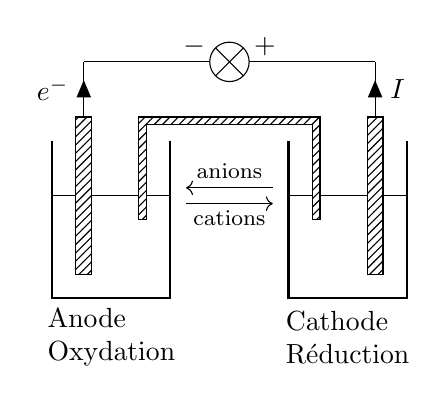
\begin{tikzpicture}[baseline=(current bounding box.north),cross/.style={path picture={ 
  \draw[black]
(path picture bounding box.south east) -- (path picture bounding box.north west) (path picture bounding box.south west) -- (path picture bounding box.north east);
}}, middlearrow/.style 2 args={
        decoration={             
            markings, 
            mark=at position 0.5 with {\arrow[xshift=3.333pt]{triangle 45}, \node[#1] {#2};}
        },
        postaction={decorate}
    }]

        % B1
        \draw[thick] (0,2) -- (0,0) -- (1.5,0) -- (1.5,2);
        \draw (0,1.3) -- (1.5,1.3);
        \draw[fill=white] (0.3,0.3) rectangle ++(0.2,2);
        \draw[fill, pattern=north east lines] (0.3,0.3) rectangle ++(0.2,2);

        % B2
        \draw[thick] (3,2) -- (3,0) -- (4.5,0) -- (4.5,2);
        \draw (3,1.3) -- (4.5,1.3);
        \draw[fill=white] (4,0.3) rectangle ++(0.2,2);
        \draw[fill, pattern=north east lines] (4,0.3) rectangle ++(0.2,2);

        % Pont salin
        \draw[fill=white] (1.2,1) -- ++(0,1.2) -- ++(1.5+2*0.3,0) -- ++(0,-1.2) -- ++(0.1,0) -- ++(0,+1.2+0.1) -- ++(-1.5-2*0.3-2*0.1,0) -- ++(0,-1.2-0.1) -- cycle;
        \draw[fill, pattern=north east lines] (1.2,1) -- ++(0,1.2) -- ++(1.5+2*0.3,0) -- ++(0,-1.2) -- ++(0.1,0) -- ++(0,+1.2+0.1) -- ++(-1.5-2*0.3-2*0.1,0) -- ++(0,-1.2-0.1) -- cycle;

        % Fils elec
          \draw[middlearrow={left=2pt}{$e^-$}] (0.4,2.3) -- (0.4,3);
          \draw (0.4,3) -- (4.1,3);
          \draw[middlearrow={right=2pt}{$I$}] (4.1,2.3) -- (4.1,3);
          \node [draw,circle,cross,minimum width=0.5cm,fill=white](B) at (9/4,3){}; 

        % Arrows
        \draw[<-] (1.7,1.4) -- node[above] {\footnotesize anions} (2.8,1.4);
        \draw[->] (1.7,1.2) -- node[below=-1pt] {\footnotesize cations} (2.8,1.2);topsep=0pt
        \node at (1.8,3.2) {$-$};
        \node at (2.7,3.2) {$+$};

        \node at (3/4,-.5) {\parbox{\widthof{Oxydation}}{Anode\\Oxydation}};
        \node at (3+3/4,-.5) {\parbox{\widthof{Réduction}}{Cathode\\Réduction}};

    \end{tikzpicture}
    \end{wrapfigure}

Elle repose sur le transfert indirect d'électrons lors de réactions d'oxydoréduction: les deux compartiments de la pile sont constitués d'une électrode plongée dans un électrolyte, les deux formant un couple redox. Pour s'effectuer, la réaction nécessite un transfert d'électrons entre les deux compartiments de la pile qui est permis par un fil métallique reliant les électrodes. Un pont salin est présent entre les compartiments pour équilibrer les charges des solution et ainsi fermer le circuit, permettant à la pile de fonctionner (les ions qu'il contient vont migrer vers un compartiment en fonction de leur signe, et ainsi \say{combler (ou laisser) la place d'un ion} de la solution impliqué dans la réaction). Au cours de son fonctionnement, la pile se rapproche de l'équilibre, i.e. $Qr \to K$.

\vspace{0.4em}
\subsection{Capacité électrique}
C'est la charge électrique totale que peut débiter la pile durant sa vie. Elle vaut
\[
  Q_{max}=n_{\text{\ce{e^-}}}\cdot N_A \cdot e = n_{\text{\ce{e^-}}} \cdot F \quad\text{ où }\quad F=N_A\cdot e \quad\text{ est la constante de Faraday}
\]
On peut trouver $n_{\text{\ce{e^-}}}$ grace à une des deux demi-réactions impliquées.

\vspace{0.4em}
\subsection{Électrolyse}
On peut inverser le sens d'évolution d'un système en lui apportant de l'énergie. L'électrolyse exploite ce fonctionnement, en apportant l'énergie grace à un générateur électrique. On peut effectuer un bilan de matière à l'aide de la relation précédente, en prenant $Q=I\cdot\Delta T$.

\vspace{0.4em}
\section{Transformations nucléaires}
On note un noyau \ce{^A_ZX}, où \ce{X} est le symbole de l'élément, \ce{^A} est le \textbf{nombre de masse} (nombre de nucléons), et \ce{_Z} le \textbf{numéro atomique} (nombre de protons). Deux noyaux ayant le même nombre de protons mais un nombre différent de nucléons sont dits \textbf{isotopes}.

\vspace{0.4em}
\subsection{Désintégration radioactive}
 La radioactivité est la désintégration \textbf{naturelle, aléatoire} et \textbf{spontanée} de noyaux, libérant une particule et de l'énergie. Lors d'une désintégration, les \textit{lois de soddy} s'appliquent:
 \begin{itemize}[topsep=0pt, noitemsep, leftmargin=*]
   \item Conservation du nombre de masse (total de \ce{^A}).
   \item Conservation du nombre de charges électriques (total de \ce{_Z}).
 \end{itemize}

\vspace{0.4em}
 \subsection{Types de radioactivité}
 \newlength{\minuslength}
 \setlength{\minuslength}{\widthof{\ce{_{-}}}}
 {\renewcommand{\arraystretch}{1.5}
\begin{tabular}{ |l|l|l|l|}
  \hline
  \textbf{Radioactivité} & \textbf{Particule émise} & \textbf{Symbole} & \textbf{Équation de la désintégration}\\
  \hline
  $\alpha$ & Noyau d'hélium 4 & \ce{^4_2He} & \ce{^A_ZX -> ^{A-4}_{Z-2}Y + ^4_2He \;( + \gamma)}\\
  $\beta^-$ & Électron & \hspace{-\minuslength}\ce{^0_{-1}e} & \ce{^A_ZX -> ^A_{Z+1}Y + ^0_{-1}e ( + \gamma)}\\
  $\beta^+$ & Positon & \ce{^0_1e} & \ce{^A_ZX -> ^A_{Z-1}Y + ^0_1e ( + \gamma)}\\
  \hline
\end{tabular}}\\
Après une désintégration, le noyau obtenu se trouve généralement dans un état exité. Pour gagner en stabilité, il émet un photon de haute énergie (émission gamma).

\vspace{0.4em}
\subsection{Diagramme (N,Z)}
\begin{wrapfigure}[9]{r}{0.5\textwidth}
  \vspace{-3em}
  % Thanks to David ALBERTO for the plot (https://www.astrolabe-science.fr/diagramme-n-z-nucleides-latex/).
  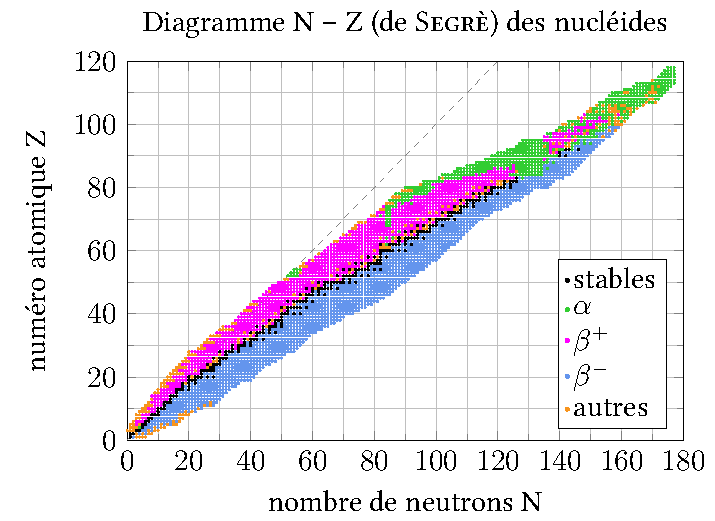
\includegraphics[width=0.5\textwidth, angle=0]{./DiagrammeNZ/diagramme_NZ.pdf}
\end{wrapfigure}
Représente les noyaux et leurs isotopes par leur numéro atomique et nombre de masse. Sur le graphique ci-contre, une ligne représente les isotopes. Généralement, les noyaux en excès de neutrons subissent une désintégration $\beta^-$, ceux en excès de protons une désintégration $\beta^+$, et les noyaux lourds, une désintégration $\alpha$. La zone stable s'app. \say{vallée de la stabilité}.

\vspace{0.4em}
\subsection{Activité}
L'activité $A$ en Becquerel d'un échantillon est le nombre de désintégrations par seconde.
  \[
    A(t)=-\frac{dN(t)}{dt}
  \]
  Selon la loi de décloissance radioactive, elle est proportionnelle au nombre de noyaux:
  \[
    A(t)=\lambda N \implies N(t)=N_0 e^{-\lambda t} \implies t_{\nicefrac{1}{2}}=\frac{\ln 2}{\lambda}
  \]
  
\vspace{0.4em}
\section{Modélisation microscopique de l'évolution d'un système}
\begin{itemize}[noitemsep, leftmargin=*]
  \item Une transformation chimique peut être représentée comme la succession d'\textbf{actes élémentaires}, événement à l'échelle microscopique qui correspond à un choc entre deux entités, entrainant la rupture ou la formation de liaisons.
  \item Un \textbf{mécanisme réactionnel} est l'ensemble des actes élémentaires d'une réaction.
  \item Les \textbf{intermédiaires réactionnels} sont produits puis consommés lors de la réaction et \textbf{n'interviennent pas dans l'équation bilan}.
  \item Un \textbf{catalyseur} modifie le mécanisme réactionnel (remplace une étape lente par plusieures rapides). Consommé puis totalement regénéré, il n'apparaît pas dans l'équation bilan.
\end{itemize}

\subsection{Sites donneurs et accepteurs de doublets d'électrons}
\begin{itemize}[noitemsep, leftmargin=*]
  \item \textbf{Site donneur}: site riche en électrons (\textit{doublet non liant, laison polarisée ou double...}).
  \item \textbf{Site accepteur}: atome en déficit d'électrons (\textit{charge positive partielle ou non, lacune...}).
\end{itemize}

\subsection{Formalisme des flèches courbes}
\begin{wrapfigure}{r}{5cm}
  \centering
  \vspace{-1.5em}
\schemestart
\chemfig[angle increment=90, atom sep=2em]{@{dnl}\charge{45:4pt=\tiny$\ominus$,0=\|,-90=\|,180=\|,90=\|}{I}}
\quad\+\quad
\chemfig[angle increment=90, atom sep=2em]{H-C-@{b1}C(-[1]H)(-[@{a2}]@{b2}\charge{90=\|,0=\|,-90=\|}{Cl})(-[-1]H)}
\schemestop
\chemmove{
\draw[green,shorten <=5pt,shorten >=1pt] (dnl).. controls +(-20:1.5cm) and +(-140:1cm).. (b1);
\draw[red,shorten <=3pt,shorten >=1pt] (a2).. controls +(90:0.5cm) and +(135:0.3cm).. (b2);
}
\end{wrapfigure}
On représente le mouvement d'un doublet d'électron ou cours d'un acte élémentaire par une flèche courbe, \textbf{orientée du site donneur au site accepteur} . Ces flèches modélisent la formation et la rupture d'une liaison au cours d'une transformation chimique.\\

\end{document}
